\documentclass[a4paper, 12pt]{extarticle}
\usepackage[utf8]{inputenc}

\usepackage{float}
\usepackage{graphicx}
\usepackage{hyperref}
\usepackage{parskip}
\usepackage{booktabs}
\usepackage{caption}
\usepackage{enumitem}
\usepackage{amsmath}
\usepackage{tabularx}
\usepackage{booktabs}
\usepackage{amsfonts}
\usepackage{multirow}

\usepackage{biblatex}
\addbibresource{main.bib}


% >= 3.45cm is too large to fit 2 names per row
\usepackage[left=2cm,right=2cm,top=3cm,bottom=3cm]{geometry}


\title{
    CITS4404 Team Project - Building AI Trading Bots
    \\ \large Group 6 - Part II: Report
    \\ 2855 Words
}
\author{
    Chen, Zijian\\
    \normalsize \texttt{22998691@student.uwa.edu.au}
    \and
    Dai, Ethan\\
    \normalsize \texttt{23625929@student.uwa.edu.au}
    \and
    Ida Bagus Prawira Janottama Kn\\
    \normalsize \texttt{23894575@student.uwa.edu.au}
    \and
    Nadeesha Adikari\\
    \normalsize \texttt{24041382@student.uwa.edu.au}
    \and
    Su, Daniel\\
    \normalsize \texttt{22965999@student.uwa.edu.au}
    \and
    Townshend, Nathan\\
    \normalsize \texttt{22970882@student.uwa.edu.au}
}

\date{}


\begin{document}

\maketitle

\begin{abstract}
    \noindent
    This report focuses on the application and investigation into the Artificial Bee Colony and Particle Swarm Optimisation with Simulated Annealing algorithms, both derived from Particle Swarm Optimisation, on optimising a Bitcoin trading bot. The bot's trading signal is calculated based on several moving averages, with the algorithms used to find the optimal parameters which control the moving average windows, and the relative importance of each of our moving average based features.\\
    
    \noindent
    Our code implementation can be seen in the following GitHub repository:\\ \href{https://github.com/DominiAetheres/cits-4404-project}{https://github.com/DominiAetheres/cits-4404-project}
\end{abstract}

\newpage
\tableofcontents

\newpage
\section{Introduction}
The increasing volatility and complexity of cryptocurrency markets, particularly Bitcoin, present a compelling challenge for algorithmic trading systems \cite{dakalbab2024artificial}. This project aims to address this challenge by developing AI-powered trading bots capable of making intelligent buy, sell, and hold decisions based on technical indicators and historical price patterns. The focus of this phase is to implement and evaluate trading strategies optimised by nature-inspired algorithms, using historical Bitcoin OHLCV data spanning several years. 

For Deliverable 2, mainly two algorithms were selected from our prior research:  Modified Particle Swarm Optimisation with Simulated Annealing (PSO-SA) and the Artificial Bee Colony (ABC) algorithm. All two methods are rooted in swarm intelligence and have demonstrated robust search capabilities across diverse optimisation problems. PSO was implemented as a useful baseline for comparison. 

The PSO-SA algorithm combines Particle Swarm Optimisation's global search with Simulated Annealing's local refinement, making it well-suited for tuning technical indicators in noisy, dynamic financial markets \cite{psosa}. The Artificial Bee Colony (ABC) algorithm, inspired by honeybee foraging, balances exploration and exploitation through a decentralised process involving employed, onlooker, and scout bees, offering a simple yet effective approach to optimising multi-parameter trading strategies \cite{abc}. 

This report outlines the implementation of optimisation algorithms to optimise a rule-based trading strategy using technical indicators such as Simple Moving Average (SMA), Exponential Moving Average (EMA) and Linear-weighted moving average (LMA). The trading bots are trained on historical data and evaluated on unseen test data, with performance measured based on the final cash value held at the end of the simulation, reflecting the profitability of the strategy. 

\newpage

\section{Overview of Investigated Algorithms}

\begin{table}[H]
    \centering
    \begin{tabularx}{\textwidth}{X X}
      \toprule
      \textbf{Algorithm} & \textbf{Description}\\
      \midrule
      Particle Swarm Optimisation with Simulated Annealing (PSO-SA) \cite{psosa} & Combines Particle Swarm Optimisation (PSO) \cite{pso} with Simulated Annealing (SA) to increase the probability of exploration of the search space. It accepts new positions for particles that are worse depending on the Metropolis effect as part of SA. \\
      Grey Wolf Optimiser (GWO) \cite{wolf} & Emulates the social hierarchy of grey wolves. The fitness of the particles decides the seniority of each of the individuals. In the update step, particles are drawn more strongly to more senior individuals. This means the search is dependent on the top few positions rather than a single best.\\
      Gravitational Search Algorithm (GSA) \cite{GSA} & Each particle within the swarm is assigned a gravitational value based on its fitness. Position updates are calculated based on the sum of the gravitational pull with all other bodies.\\
      Harris Hawks Optimiser (HHO) \cite{hawks} & Emulates the hunting behaviour of Harris Hawks. Individuals searching a large area before selecting specific areas to exploit.\\
      Artificial Bee Colony (ABC) \cite{abc} & Models the roles of bees within a hive. The idea is to split the individuals into multiple roles which fulfils exploration and exploitation of the search space at the same time.\\
      Firefly Algorithm (FA) \cite{firefly}& Inspired by fireflies and uses distance as a factor for convergence. Each individual has a brightness based on their fitness, and attraction is dependent on both brightness and distance away from the corresponding particle.\\ 
      \bottomrule
    \end{tabularx}
    \caption{Summary of the algorithms which were covered in the preceding literature review.}
    \label{tab:algorithms}
  \end{table}

\newpage
\section{Bot Design and Parameterisation}
Bitcoin as an asset is fundamentally unlike other classes of assets. It is a currency rather than a stock and is consequently closer to foreign exchange trading rather than stock trading. There are few, if any, fundamental indicators for Bitcoin making it disproportionately impacted by naked supply and demand. This was especially true in its early days as it hadn't yet gained a reputation amongst younger investors as the trendy new replacement for gold as a store of value. Thus, common technical analysis indicators were chosen as inputs for the trading signal. 

Three moving averages common in technical analysis \cite{brock1992simple} are included in the trading signal informing the bot: 

\begin{itemize}
    \item Simple moving average (SMA) 
    \item Exponential moving average (EMA) 
    \item Linear-weighted moving average (LMA) 
\end{itemize}

Different moving averages have sensitivities to different behaviours in the market. The SMA weighs all historical data points equally resulting in an indicator which is more resistant to market volatility. Both EMA and LMA place a heavier weight on more recent data points with the former having an exponential weighting to more recent data points compared to the linear weighting of the latter. EMA is more prone to following the market while LMA provides a middle ground between SMA and EMA. 

These three moving averages form two trading signal components: 

\begin{enumerate}
    \item SMA $-$ EMA 
    \item EMA $-$ LMA 
\end{enumerate}

Both differences between averages seek to measure the deviation of the market from the mean, where a crossover is indicative of a potential change in market direction. The first is more sensitive to market fluctuations as SMA carries far more momentum due to its equal weighting of its data points where the second is a more detailed indicator of market direction as their crossovers would provide information into shorter term variations in price direction. 

During the training loop, the number of days for each of the above moving averages is optimised. The momentum of each of the averages, calculated as daily deltas, are also factored into the trading signal, allowing it to capture some information about their movement and volatility: 

\begin{enumerate}[start=3]
    \item SMA momentum 
    \item EMA momentum 
    \item LMA momentum 
\end{enumerate}

\newpage
The information provided to the trading bot may not be equally important to the final trading signal. In recognition of this, five weight parameters were added which control the strength of each of the above five indicators. 

\begin{enumerate}[start=6]
    \item SMA - EMA weight 
    \item EMA - LMA weight 
    \item SMA momentum weight 
    \item EMA momentum weight 
    \item LMA momentum weight 
\end{enumerate}

\begin{table}[H]
    \centering
    \begin{tabularx}{\textwidth}{X X X}
      \toprule
      \textbf{Parameter} & \textbf{Domain} & \textbf{Description} \\
      \midrule
      SMA window        & $\in \mathbb{Z}^+$, (0, 100]  & Window for the calculation of SMA \\
      EMA window        & $\in \mathbb{Z}^+$, (0, 100]  & Window for the calculation of EMA   \\
      LMA window        & $\in \mathbb{Z}^+$, (0, 100]  & Window for the calculation of LMA   \\
      EMA $\alpha$      & $\in \mathbb{R}$, (0, 1)  & Used as weight decay rate term for calculating EMA\\
      $w_1$             & $\in \mathbb{R}$, [0, 100]  & Weighting for SMA-EMA term \\
      $w_2$             & $\in \mathbb{R}$, [0, 100]  & Weighting for EMA-LMA term  \\
      $w_3$             & $\in \mathbb{R}$, [0, 100]  & Weighting for SMA momentum term \\
      $w_4$             & $\in \mathbb{R}$, [0, 100]  & Weighting for EMA momentum term\\
      $w_5$             & $\in \mathbb{R}$, [0, 100]  & Weighting for LMA momentum term \\
      $\theta$          & $\in \mathbb{R}$, [0, 500]  & Threshold for clamping signal to {-1, 1}  \\
      \bottomrule
    \end{tabularx}
    \caption{Parameters that are optimised for the trading bot.}
    \label{tab:parameters}
  \end{table}

\newpage
The final component of the trading signal is the threshold parameter $\theta$. When the signal value exceeds the positive threshold, a buy signal is triggered and vice versa. This simplifies the trading signal to a value between 1 and -1 for buy and sell respectively. The trading signal is as follows where the function $s_{raw}$ produces the unclipped trading signal at time interval $t$ and $s$ is the final clipped trading signal.

\begin{multline}
    $$ s_{raw}(t) = w_1(\text{SMA}_{t} - \text{EMA}_{t}) + w_2(\text{EMA}_{t} - \text{LMA}_{t}) + \\
    w_3(\text{SMA}_t - \text{SMA}_{t - 1}) + w_4(\text{EMA}_t - \text{EMA}_{t - 1}) + w_5(\text{LMA}_t - \text{LMA}_{t - 1}) $$
\end{multline}

\begin{equation}
s(t) = 
\begin{cases}
1,      & s_{raw}(t) > \theta,\\
-1,     & s_{raw}(t) < -\theta.
\end{cases}
\end{equation}

There are ten total parameters which are optimised for use by the bot (Table \ref{tab:parameters}). These vary the time windows for the calculation of the moving averages and impact the moving average values within function (1).

\section{Algorithm Selection and Implementation}
Both ABC and PSO-SA can trace their lineages to the original PSO algorithm. PSO was the initial introduction of a nature-inspired optimisation algorithm based on the flocking or swarming behaviour of animals such as birds or fish. PSO is suited to domains with high dimensionality due to its computational efficiency compared to methods based on genetic algorithms. The time available to investigate and tune our models was limited which was a factor in the decision to select PSO-based algorithms. 

Early convergence due to a bias towards exploitation rather than exploration is a common issue with PSO. Although the magnitude of velocity updates of the individuals are random, the direction are always towards a combination of global best and personal best depending on the hyperparameters chosen. ABC and PSO-SA both address this by increasing the amount of exploration performed in the search space. 

The papers introducing ABC and PSO-SA have benchmarked their performance on a variety of search spaces, including high dimensional and multi-modal functions. In this report, the efficacy of the different exploration methods will be tested in comparison to basic PSO. 

Our implementation of each of these algorithms can be found at:\newline
\href{https://github.com/DominiAetheres/cits-4404-project}{https://github.com/DominiAetheres/cits-4404-project}.

\begin{figure}[H]
    \centering
    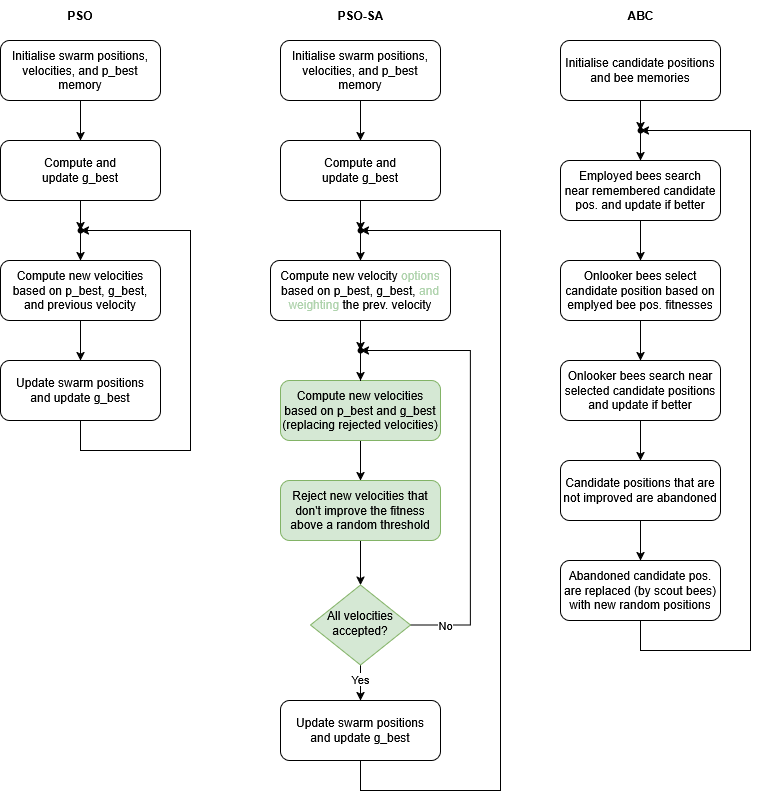
\includegraphics[width=0.76\textwidth]{./assets/opt_alg.png}
    \caption{Flowcharts for the three implemented algorithms.}
    \label{fig:alg-flowchart}
\end{figure}

Note: in Figure \ref{fig:alg-flowchart}, the PSO-SA sections in green are the modifications made to PSO.

\subsection{ABC} 
ABC splits the swarm population into three distinct roles which focus on either exploration or exploitation: 

\begin{enumerate}
    \item Employed bees exploit around known best positions and employs a neighbourhood search to improve their positions. 
    \item Onlooker bees assess the quality of solutions based on the information gathered by employed bees and select positions based on that information to explore further in the most promising known areas.
    \item Scout bees explore the search space by randomly replacing discarded positions with new ones randomly selected from the entire search space. 
\end{enumerate}

This role-based approach allows the simultaneous exploitation of the known best positions within the search space and exploration of the entire search space through random sampling. 

\subsection{PSO-SA} 
PSO-SA utilises a hybrid algorithm approach by incorporating Simulated Annealing (SA) into the new position acceptance process. When the PSO particle position update process occurs, particles have their fitness evaluated. The acceptance process uses the temperature during a particular iteration. Higher temperatures allow suboptimal updates with a higher probability which allows the initial exploration of the search space even if new positions aren't optimal, while lower temperatures encourage exploitation with lower probabilities of accepting worse new positions.   

The metropolis process is time-consuming, especially at lower temperatures as velocities and positions are repeatedly recalculated for particles which fail the acceptance criteria. Due to time constraints, our implementation contains a hard limit on how many times a particle can be recalculated during the SA loop. 

\section{Experiments and Evaluation Methodology}

This project used daily Bitcoin OHLCV (Open, High, Low, Close, Volume) data from the publicly available Bitcoin Historical Dataset on Kaggle \cite{kaggle}. The dataset spans from 2014 to 2022, offering clean and consistent daily price and volume records. We selected the full available date range to ensure sufficient variation in market conditions for both training and evaluation. Although only the daily data was used in this project, the original dataset \cite{kaggle} also includes hourly and minute-level data. 

The daily data was split into a training set (covering the years up to 2019) consisting of 1,861 data points, and a testing set (covering from 2020) with 792 previously unseen data points. This split reflects a realistic workflow in which the trading bot is optimised using historical data and then evaluated on future data to assess its generalizability and robustness. 

We employed a grid search approach to tune the strategy's hyperparameters for each optimiser (PSO, PSO-SA, ABC). Over 100 iterations, we explored combinations of values for parameters such as population size, acceleration coefficients, and others. Each candidate configuration was evaluated using a custom scoring function, which was designed to reflect desirable characteristics in a trading bot's behaviour.
The fitness of each bot was defined as the amount of cash it held at the end of the back-tested period, a direct indicator of how successful its trading strategy was under historical market conditions.

The final selected hyperparameters for each optimiser are listed in the table below. The number 42 was used as the seed in the grid search, as well as for initial training and testing.  

\begin{table}[H]
    \centering
    \label{tab:optimizers}
    \begin{tabular}{llr}
      \toprule
      \textbf{Optimiser} & \textbf{Hyper-parameter}                          & \textbf{Value} \\ 
      \midrule
      \multirow{3}{*}{PSO}      
        & Number of agents in the swarm (\texttt{population\_size})       & 10   \\
        & Personal (cognitive) acceleration coefficient (\texttt{p\_increment}) & 0.2  \\
        & Social acceleration coefficient (\texttt{g\_increment})         & 0.1  \\
      \midrule
      \multirow{5}{*}{PSO-SA}   
        & Number of agents in the swarm (\texttt{population\_size})       & 10   \\
        & Personal acceleration coefficient (\texttt{p\_increment})      & 0.1  \\
        & Global acceleration coefficient (\texttt{g\_increment})        & 0.1  \\
        & Initial temperature for simulated annealing (\texttt{init\_temp}) & 100  \\
        & Cooling rate (\texttt{cool\_rate})                             & 0.9  \\
      \midrule
      \multirow{2}{*}{ABC}      
        & Colony Size                                                   & 10   \\
        & Position Age Limit                                            & 3    \\
      \bottomrule
    \end{tabular}
    \caption{Optimisers and discovered optimal hyperparameters}
\end{table}

Due to time and resource constraints, the grid search was performed only for a selected set of parameter values, and additional parameters would have been explored with more time and resources. The evaluation cost in optimisation algorithms like PSO, PSO-SA, and ABC is a key practical challenge. Each candidate solution requires running a trading simulation over historical data, which can be computationally expensive. The number of evaluations grows with the parameter space size and optimisation iterations. The evaluation process involves training the strategy on historical data, calculating custom performance metrics, and assessing results, leading to substantial resource usage in terms of time and memory. A major trade-off exists between exploring a broad parameter space, which can yield better results but increases evaluation time, and narrowing the search space, which reduces time but may miss optimal solutions. Given limited resources, efficient allocation is crucial. Techniques like parallel computing can help mitigate evaluation costs, but careful consideration of available resources is still needed to balance performance with practicality. 

\newpage
\section{Results and Analysis}
\subsection{Summary of Training Statistics}
We compared three population-based optimisers across training and testing phases, using daily Bitcoin OHLCV data spanning 2014-2019 for training and 2020-2022 for testing. Our primary evaluation metric was final portfolio value (cash after liquidating positions), averaged over five random seeds, with standard deviation to capture robustness. 

\begin{table}[ht]
    \centering
    \begin{tabular}{lrrr}
      \toprule
      \textbf{Algorithm} & \textbf{Training Score} & \textbf{Training Std. Dev.} & \textbf{Test Score} \\
      \midrule
      PSO     & 31353.24 & 6537.15 & 2374.42 \\
      PSO-SA  & 28283.67 & 3934.15 & 2211.53 \\
      ABC     & 25316.08 & 4262.97 & 2070.11 \\
      \bottomrule
    \end{tabular}
    \caption{Training vs. test final cash across optimisers}
    \label{tab:algorithm_scores}
\end{table}

Table \ref{tab:algorithm_scores} clearly shows that PSO achieves the highest training returns but suffers the largest drop to test, indicative of overfitting. PSO-SA strikes a middle ground—slightly lower training performance than PSO but more consistent test results. ABC is the most conservative: lowest training and test values, but a modest train-test gap. 

\subsection{Algorithm Behaviour}
\subsubsection{Convergence Behaviour}

\begin{figure}[h!]
    \centering
    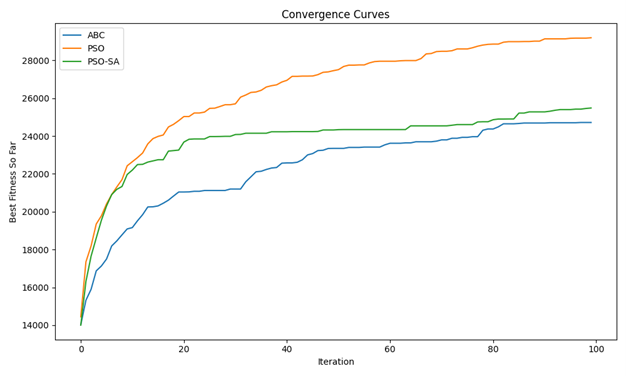
\includegraphics[width=0.8\textwidth]{./assets/convergence.png}
    \caption{Average Convergence Curves}
    \label{fig:convergence}
\end{figure}

In Figure 1, PSO shows the steepest initial ascent but quickly plateaus at a suboptimal fitness on the test set. ABC climbs more gradually with low inter-seed variance. PSO-SA follows PSO's rapid rise in early iterations, then leverages a Metropolis acceptance (simulated annealing) to escape local traps and achieve the highest final fitness with the tightest clustering. 

\subsubsection{Robustness}
Measured by training-set standard deviation across seeds (PSO $\approx$ 6537, ABC $\approx$ 4263, PSO-SA $\approx$ 3934),  PSO-SA consistently exhibits the lowest variability in both training and test returns, making it the most repeatable. ABC sits in the middle—its scout phase injects diversity but also yields moderate scatter. Pure PSO, lacking any "escape" mechanism, is prone to getting stuck; one unlucky seed can drastically underperform. 

\subsubsection{Exploration vs. Exploitation}
\begin{enumerate}
    \item    \textbf{PSO}: Inertia-cognitive-social updates provide broad early exploration, but once particles converge on the global best they rarely deviate, leading to premature stagnation. 
    \item     \textbf{ABC}: Alternates exploitation (employed/onlooker bees refining known sources) with exploration (scout bees randomly seeding new positions), maintaining diversity at the cost of slower convergence. 
    \item     \textbf{PSO-SA}: Adds a Metropolis acceptance rule to PSO's velocity update. High “temperature” early on allows uphill moves (exploration); as temperature cools, it reverts to pure PSO (exploitation). This dynamic schedule balances global search and local refinement. 
\end{enumerate}

\subsubsection{Equity Curves}
\begin{figure}[h!]
    \centering
    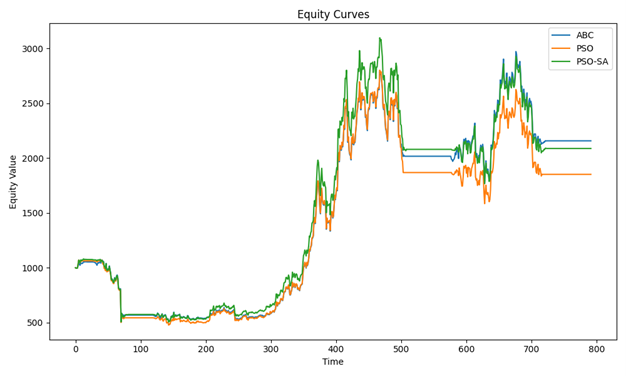
\includegraphics[width=0.8\textwidth]{./assets/equity.png}
    \caption{Average Equity Curves}
    \label{fig:equity}
\end{figure}
Figure \ref{fig:equity} shows the mean portfolio value over the unseen test period. PSO-SA delivers the smoothest equity growth - smaller drawdowns and steady gains. PSO's curve is far more jagged, echoing its over-sensitivity to initial seeds. ABC yields the flattest, most conservative growth. 

\newpage
\subsubsection{Indicator Evolution}

We visualise how the learned thresholds and buy/sell signals evolve on the same test series for each algorithm, show how the buy/sell indicator toggles between +1, -1, and 0 over time. PSO-SA's signal exhibits balanced responsiveness: it captures major up-trends and down-trends without excessive whipsaws. PSO generates more frequent, erratic flips, explaining its higher transaction count and associated slippage. ABC produces sparser signals, often missing shorter trend reversals. 

The trading signal figures for this section are provided in the Appendix. Only the first signal in a series of recurring signals is executed. If there are multiple repeating buy signals, the asset is held. The reverse is true for sell signals.

All three algorithms capture the major Bitcoin uptrends, but PSO often chases minor fluctuations (many small trades), consistent with its overfitting. ABC trades less frequently, while PSO-SA provides a middle ground. 

\begin{figure}[H]
    \centering
    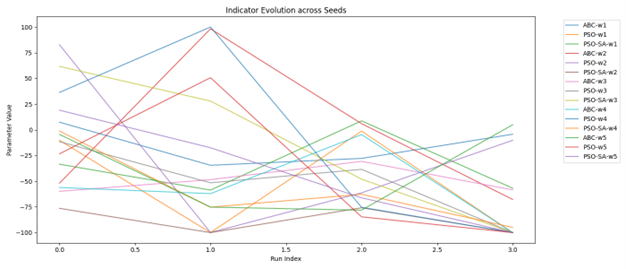
\includegraphics[width=\textwidth]{./assets/parameter_weights.png}
    \caption{Parameter evolution}
    \label{fig:parameter}
\end{figure}
Figure \ref{fig:parameter} tracks five key momentum weights (w1-w5) across seeds for each algorithm's best solution per run. ABC's weights fluctuate most dramatically (due to its scout resets). PSO-SA's curves are the smoothest, signalling highly consistent parameter choices. PSO shows sporadic jumps, reflecting its greedy no-escape policy. 

\newpage
\subsubsection{Parameter Sensitivity}
We inspected correlations amongst the ten learned hyperparameters (averaged over seeds and algorithms).
\begin{figure}[H]
    \centering
    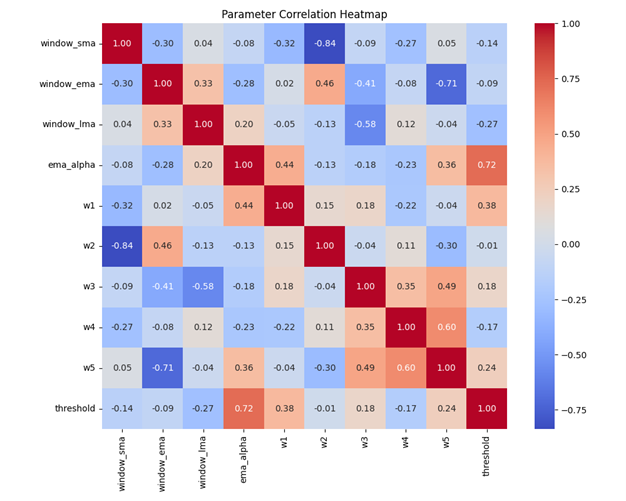
\includegraphics[width=\textwidth]{./assets/sensitivity.png}
    \caption{Parameter correlation heatmap}
    \label{fig:sensitivity}
\end{figure}
Figure \ref{fig:sensitivity} reveals pairwise correlations amongst the ten optimised parameters. A striking -0.84 correlation between \texttt{window\_sma} and $w_2$ (EMA$-$LMA difference weight) suggests that longer SMA windows are systematically offset by more negative momentum weights. Such insights can drive more efficient future grid searches by pruning redundant dimensions. 


\newpage
\section{Conclusion}
In this project, we successfully implemented and evaluated three nature-inspired algorithms: Particle Swarm Optimisation (PSO), PSO with Simulated Annealing (PSO-SA), and Artificial Bee Colony (ABC) for optimising a rule-based Bitcoin trading bot. The core objective was to use these algorithms to find effective parameters for a trading strategy based on Simple, Exponential, and Linear-Weighted Moving Averages (SMA, EMA, LMA). Quantitatively, while PSO achieved the highest average training score (31353.24), its test score (2374.42) was comparable to PSO-SA (2211.53, with a lower training standard deviation of 3934.15) and ABC (2070.11), suggesting challenges in generalisation to new market conditions.

The project found that standard PSO converges quickly onto extrema. In contrast, PSO-SA and ABC tended to converge more slowly overall as they traded off immediate exploitation for a broader search. While PSO's faster initial convergence might be advantageous for simpler search spaces, the exploration of PSO-SA and ABC can be important for tackling complex optimisation problems. It turned out that our search space may have been relatively simple, or too limited as PSO performed the best by immediately exploiting to the best solution.

Defining the search space by parameterising indicator window sizes and weights resulted in a high-dimensional problem, and we also learned about some interdependencies between these parameters. The performance was sensitive not only to the algorithm's effectiveness but also to the choice of indicators and the structure of the trading rules. Financial data often changes its patterns over time, making it difficult for strategies optimised on past data to remain consistently effective, illustrating the limitations of back-testing.

For future work, several paths could be explored. Testing the optimised bots in a live trading simulation would provide further insights into their reliability. Better results might be achieved by incorporating more advanced indicators or features, or by exploring other algorithms from Part 1 (e.g., GWO, HHO). Furthermore, refining the evaluation to include consistency metrics, such as the standard deviation of scores, in addition to the final profit, may lead to more robust and reliable trading strategies. 

\newpage
\printbibliography

\newpage
\appendix
\section{Trading Signals for PSO}
\begin{figure}[h!]
    \centering
    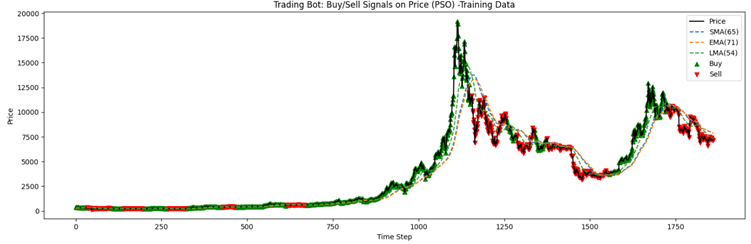
\includegraphics[width=\textwidth]{./assets/pso_train.png}
\end{figure}
\begin{figure}[h!]
    \centering
    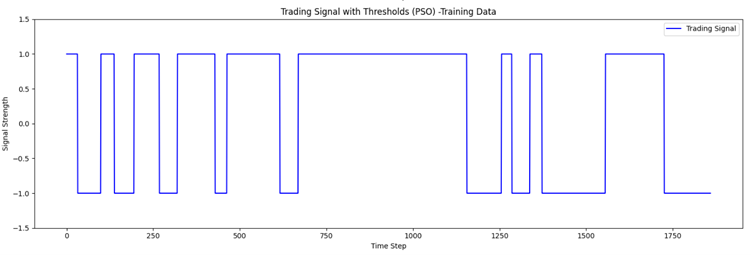
\includegraphics[width=\textwidth]{./assets/pso_train_signal.png}
    \caption{The trading signal and matching points on the price graph for the \textbf{training} set.}
\end{figure}
\newpage
\begin{figure}[h!]
    \centering
    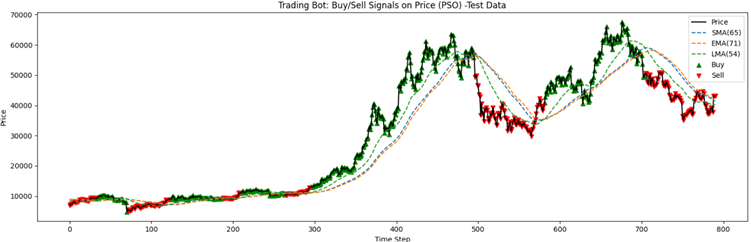
\includegraphics[width=\textwidth]{./assets/pso_test.png}
\end{figure}
\begin{figure}[h!]
    \centering
    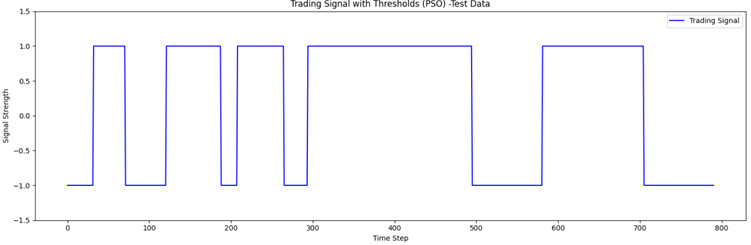
\includegraphics[width=\textwidth]{./assets/pso_test_signal.png}
    \caption{The trading signal and matching points on the price graph for the \textbf{test} set.}
\end{figure}

\newpage
\section{Trading Signals for PSO-SA}
\begin{figure}[h!]
    \centering
    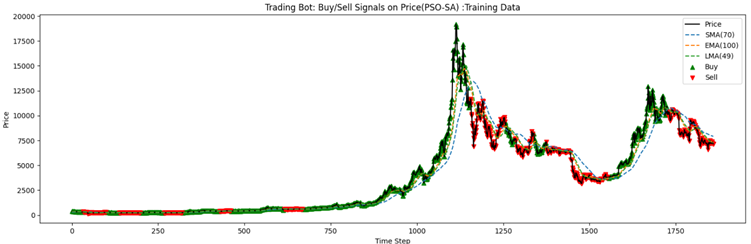
\includegraphics[width=\textwidth]{./assets/psosa_train.png}
\end{figure}
\begin{figure}[h!]
    \centering
    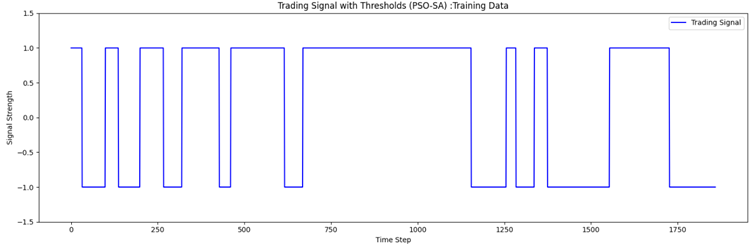
\includegraphics[width=\textwidth]{./assets/psosa_train_signal.png}
    \caption{The trading signal and matching points on the price graph for the \textbf{training} set.}
\end{figure}
\newpage
\begin{figure}[h!]
    \centering
    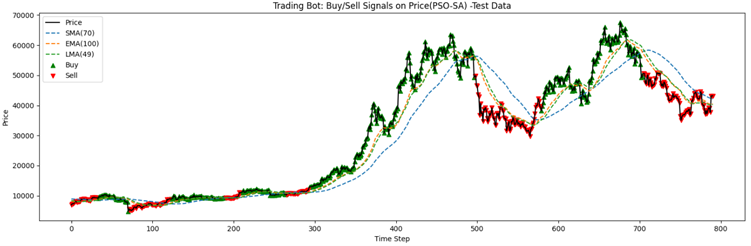
\includegraphics[width=\textwidth]{./assets/psosa_test.png}
\end{figure}
\begin{figure}[h!]
    \centering
    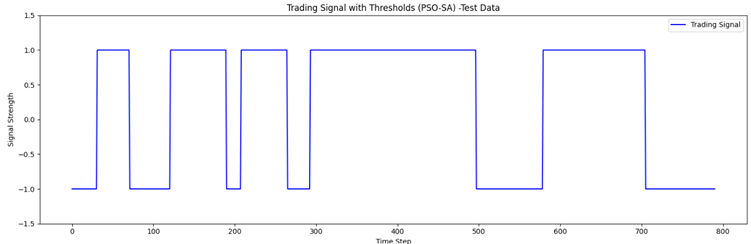
\includegraphics[width=\textwidth]{./assets/psosa_test_signal.png}
    \caption{The trading signal and matching points on the price graph for the \textbf{test} set.}
\end{figure}

\newpage
\section{Trading Signals for ABC}
\begin{figure}[h!]
    \centering
    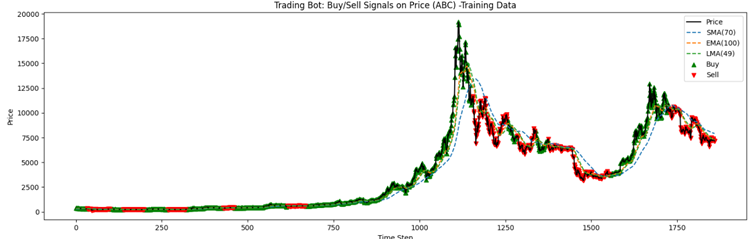
\includegraphics[width=\textwidth]{./assets/abc_train.png}
\end{figure}
\begin{figure}[h!]
    \centering
    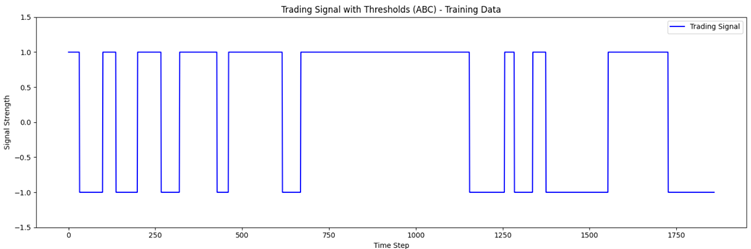
\includegraphics[width=\textwidth]{./assets/abc_train_signal.png}
    \caption{The trading signal and matching points on the price graph for the \textbf{training} set.}
\end{figure}
\newpage
\begin{figure}[h!]
    \centering
    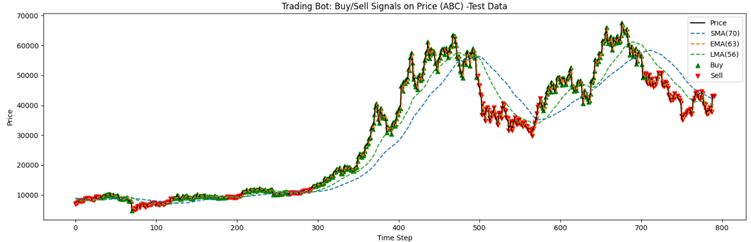
\includegraphics[width=\textwidth]{./assets/abc_test.png}
\end{figure}
\begin{figure}[h!]
    \centering
    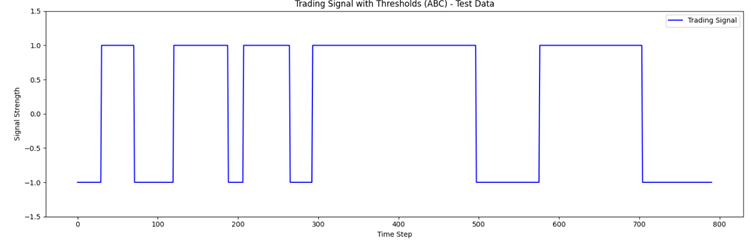
\includegraphics[width=\textwidth]{./assets/abc_test_signal.png}
    \caption{The trading signal and matching points on the price graph for the \textbf{test} set.}
\end{figure}


\end{document}